Este manual pretende introducir a los usuarios en el manejo del
software de simulación numérica Distributed and Unified Numerics
Environment (\textsc{Dune}), que se puede ubicar en la dirección
\url{https://dune-project.org}, proyecto de código abierto que
proporciona una infraestructura flexible y modular para la solución
de ecuaciones diferenciales parciales.

\section{Configuración en la nube}

Para correr el software \textsc{Dune}, vamos a utilizar el
repositorio en GitHub
\url{https://github.com/cpp-review-dune/dune-learn},
diseñado para funcionar en la nube, utilizando las ventajas que nos
ofrece \url{https://www.gitpod.io}, en él se utiliza una imagen
docker prediseñada basada en la distribución GNU/Linux
\href{https://archlinux.org}{Arch Linux}, que contiene las
dependencias y repositorios necesarios para su funcionamiento.
\footnote{
	La extensión de gitpod puede ser instalada dependiendo del
	navegador que se utilice
}
Ver la figura~\ref{fig:github01}:

\begin{figure}[ht!]
	\centering
	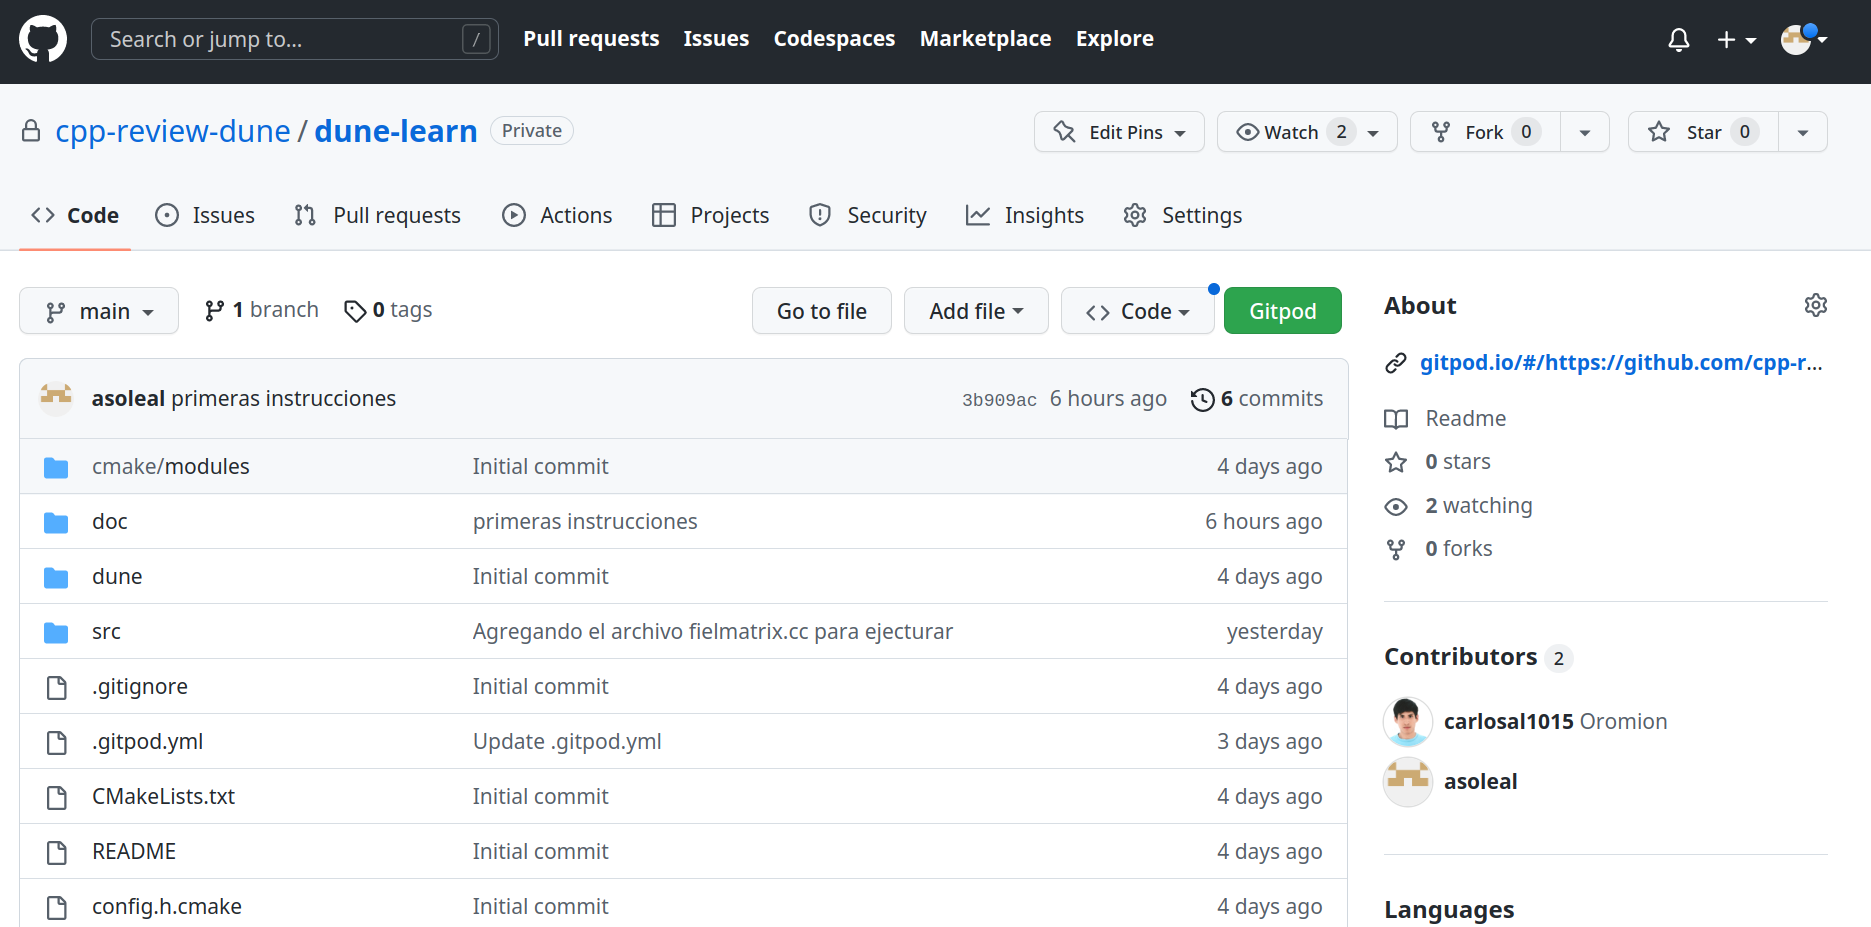
\includegraphics[scale=0.3,keepaspectratio]{cppreview-learn.png}
	\label{fig:github01}
\end{figure}

\section{Instalación}

Use el repositorio
\href{https://wiki.archlinux.org/title/Unofficial_user_repositories_(Espa%C3%B1ol)#arch4edu}{Arch Linux for Education}.
Para un mayor detalle vea.

En la sección de C++, se presentará \verb|dune-pdelab|, que fue
estudiada en el curso presentado en el año $2022$, de manera remota y
cuya link está en:
\url{https://dune-pdelab-course.readthedocs.io/en/latest/intro.html},
y en la sección de Python, utilizaremos
\href{https://jupyter.org}{JupyterLab} para introducir el uso de \verb|dune-fem|.